\scanpage{72}
\mspage{\handwritten{- 7 -}}

p.25, li.10 du bas : hint pour ``il n'est pas difficile de montrer ...''?

p.26, li.10 : ``dont on peut penser que c'est le même ...'' : y a-t-il
\figure{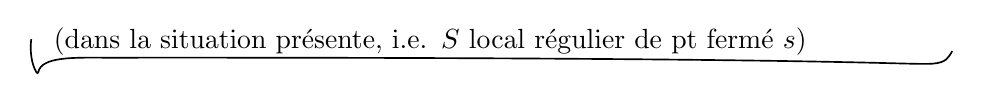
\begin{tikzpicture}
\node[inner sep=0pt,text width=0.92\linewidth,align=left] (addition)
  {\inserted{(dans la situation présente, i.e. $S$ local régulier de pt fermé $s$)}};
\handwritten{\draw[semithick]
  ([xshift=-0.8em,yshift=1.4ex]addition.south west)
  .. controls ([xshift=-0.9em,yshift=-0.3ex]addition.south west)
  and ([xshift=-0.6em,yshift=-1.7ex]addition.south west)
  .. ([xshift=-0.55em,yshift=-1.4ex]addition.south west)
  .. controls ([xshift=-0.45em,yshift=0ex]addition.south west)
  and ([xshift=0.8em,yshift=-0.15ex]addition.south west)
  .. ([xshift=2em,yshift=-0.15ex]addition.south west)
  .. controls ([xshift=-3em,yshift=-0.1ex]addition.south east)
  and ([xshift=-0.9em,yshift=-0.8ex]addition.south east)
  .. ([xshift=0em,yshift=-0.65ex]addition.south east)
  .. controls ([xshift=0.5em,yshift=-0.55ex]addition.south east)
  and ([xshift=0.55em,yshift=-0.15ex]addition.south east)
  .. ([xshift=0.7em,yshift=0.4ex]addition.south east);}
\end{tikzpicture}}
une caractérisation d'un homomorphisme (7.17.4.1) ? \handwritten{(${}^1$)}

p.27, li.1 et 2 du bas : ``au-dessus'' et non ``au dessus''. Dire ``dans le normalisé'' au lieu de ``du normalisé''.

p.28 : dans la bibliographie, manque la référence Abhyankar sur la résolution des singularités des surfaces arithmétiques.

\handwritten{(${}^1$) Est-ce que 7.2 ne \unsure{x|se} généralise pas ?}

% Unassigned detached point pair, far below the text in the lower-right blank field.
% Its punctuation value and authored status are unresolved; this is a shape record.
\margin{\raisebox{-0.36\textheight}[0pt][0pt]{\parbox{3mm}{\figure{\unsure{\begin{tikzpicture}[x=1mm,y=1mm]
\fill (0,0) .. controls (-0.22,0.07) and (-0.25,0.32) .. (-0.10,0.48)
  .. controls (0.01,0.64) and (0.29,0.45) .. (0.29,0.26)
  .. controls (0.30,0.05) and (0.14,-0.07) .. (0,0) -- cycle;
\fill (0.66,0.95) .. controls (0.45,1.00) and (0.52,1.26) .. (0.68,1.34)
  .. controls (0.81,1.43) and (0.72,1.58) .. (0.78,1.66)
  .. controls (1.02,1.52) and (1.04,1.22) .. (0.92,1.07)
  .. controls (0.85,0.96) and (0.75,0.93) .. (0.66,0.95) -- cycle;
\end{tikzpicture}}}}}}

% archive sheet number: 71
